\section{Scoring \& Evaluation}

\subsection{NCC}

\todo[inline]{NCC: Upside: Easy to create a score from, set a threshold for 'good' then just divide and give stars}
\todo[inline]{NCC: Downside: Small images lead to big score differences for seemingly small image differences}
\todo[inline]{NCC: Downside: Wasn't ranking the images in the same order that a teacher would}
\todo[inline]{NCC: Downside: Doesn't tell a student what they did wrong, just a black box score, is that all that's needed? - NO}

\subsection{HOG}

\todo[inline]{Similar to NCC, slightly more accurate but more intensive to calculate, see Delteil}

\subsection{Image Difference}

If you're handling simple 1 bit images, you can perform a simple image difference which just takes the first image, XOR'd with the second. The result (shown in Figure \ref{fig:crotchet-diff}) is a simple highlighting of the difference between the two.

\begin{figure}[h!]
  \centering
  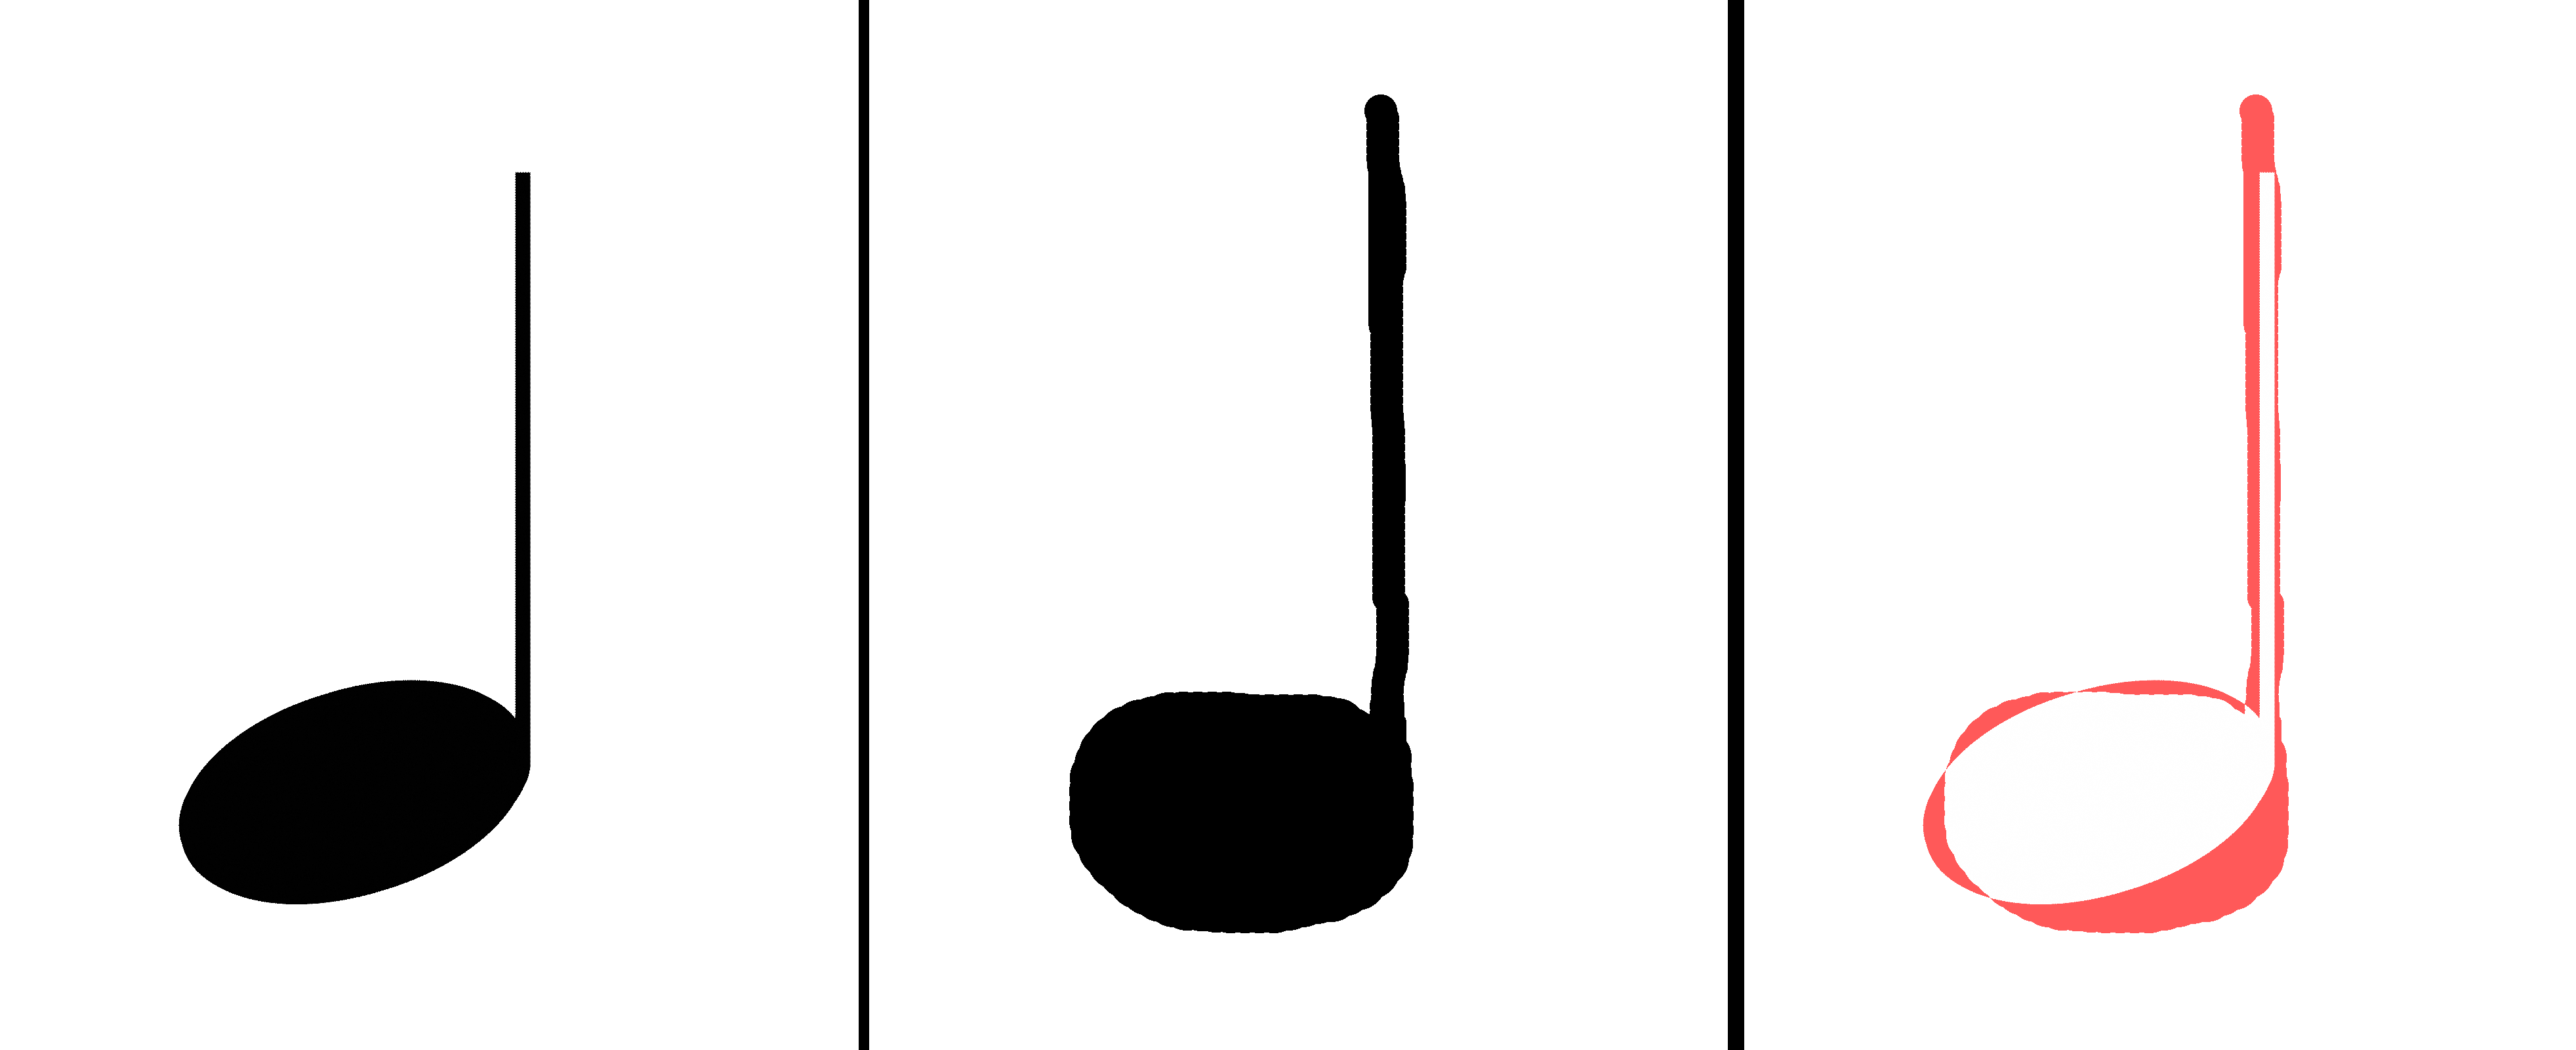
\includegraphics[width=\linewidth]{gfx/crochet-all.png}
  \caption{Highlighting differences between a perfect and a hand-drawn crochet}
  \label{crotchet-diff}
\end{figure}

\todo[inline]{Image Difference: Upside: Very visual, clear what's wrong}
\todo[inline]{Image Difference: Downside: Sensitive to the blob size, means stem errors are less likely to impact the score}